\section{Results}\label{sec:results}
In order to validate our model we ran a test with the recommended 
setup\footnote[1]{1 Godfather, 2 Mafioso, 1 Sheriff, 1 Doctor, 5 Villagers} of 3
mafia members and 7 town members\cite{MafiaRules}. This yielded a win-rate for 
each team of 
50\%. Since this 
balanced game was achieved by following the recommended rules, it seemed that 
our model indeed portrayed real games with some level of accuracy. We then ran 
experiments with a team biased toward the town\footnote{Using one of each 
town 
role from appendix \ref{app:A}, against 1 Godfather, and 2 Mafioso}. This 
yielded a win-rate of 75\% favoring the town. This was expected, further 
validating the purpose of this paper: How can one re-balance the win-rates when 
facing a powerful town. We then simulated games with every possible combination 
of mafia roles, against this baseline of a powerful town. The only 
consistent role on the mafia team was the presence of 1 Godfather. Below are 
the results: 
\begin{figure}[h]
	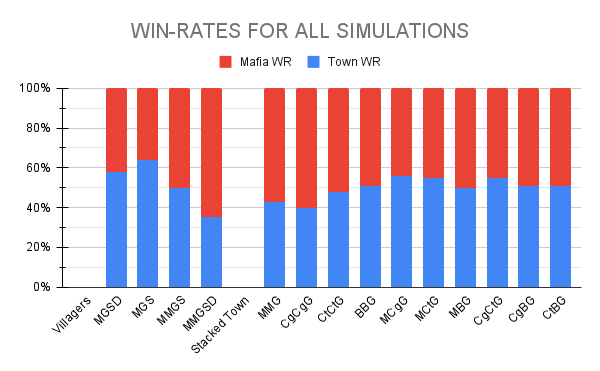
\includegraphics[width=1\linewidth]{figures/Winrates}
	\caption{\\Graph of the win-rate of various simulated game compositions.\\ 
	There were 10 players in each simulation.\\ 
	Each simulation was 100 games. 
	Simulation names are related to team composition, based on role 
	abbreviations in appendix \ref{app:A}.\\ 
	The first 4 runs labeled \textit{villager} means that all roles not 
	mentioned in the abbreviation are replaced with villagers.\\ 
	The next runs labeled \textit{stacked town} means that all roles not 
	mentioned in the abbreviation are replaced with	one of each town role.}
	\label{fig:placeholder}
\end{figure}
\\Based on this graph we can deduce that mafiosi and consiglieri are more 
impactful for the mafia than both consorts and blackmailers. But it also seems 
that the varied team consisting of one mafioso, consigliere, and Godfather, 
performs marginally better than other configurations. \\
The results indicate that when playing against a powerful town, it is more 
important for the mafia to be able to continually kill town members, and to be 
able to quickly find the most powerful roles of the town, in order to eliminate 
them, than it is to deny actions and communication to the town. \\
One can ponder that these results may be because of the limited team size of 
the game, as the blackmailer and consort roles may thrive when being able to 
use 
their actions on powerful town roles, but without enough investigative and 
murderous power behind them, they are unable to find the right targets, nor 
finish the job if they do find them. \\\\
\textbf{Section not finished due to missing data.}
